\documentclass[theme=teal]{khmermath}
\usepackage{needspace}

\geometry{left=0.8cm, right=0.8cm, top=0.35cm, bottom=0.85cm, footskip=0.58cm}
\usepackage{colortbl}
\usepackage{tikz}
\usetikzlibrary{calc,shapes,arrows,intersections,through,backgrounds,shadows,decorations.pathmorphing,angles,quotes}

% Set every math mode to display style
\everymath{\displaystyle}

% -------------------------------------------------------------------------
% Korean Math Textbook Style Color Palette & Macros
% -------------------------------------------------------------------------
\definecolor{koreaTeal}{RGB}{0, 150, 155}       % Primary Header Teal/Cyan
\definecolor{koreaDarkTeal}{RGB}{0, 105, 110}   % Dark Teal Accent
\definecolor{koreaBeige}{RGB}{247, 244, 237}     % Concept Sidebar Beige (#F7F4EE)
\definecolor{koreaBeigeBorder}{RGB}{225, 218, 205}
\definecolor{koreaOrange}{RGB}{235, 115, 30}     % Problem Number Orange
\definecolor{koreaBlue}{RGB}{35, 110, 190}      % Standard Blue
\definecolor{koreaPurple}{RGB}{125, 50, 160}    % Purple Accent
\definecolor{koreaNumber}{RGB}{115, 125, 135}   % Problem Number Gray
\definecolor{koreaYellow}{RGB}{255, 246, 175}   % Yellow Highlight Tint

\definecolor{brandNavy}{RGB}{0, 105, 110}
\definecolor{brandBlue}{RGB}{0, 150, 155}
\definecolor{brandLightBlue}{RGB}{247, 244, 237}
\definecolor{brandCrimson}{RGB}{195, 35, 60}
\definecolor{brandCoral}{RGB}{235, 80, 75}
\definecolor{brandGold}{RGB}{215, 130, 10}
\definecolor{brandGoldBg}{RGB}{255, 252, 242}
\definecolor{brandTeal}{RGB}{0, 150, 155}
\definecolor{brandTealBg}{RGB}{244, 252, 250}
\definecolor{subtleGray}{RGB}{246, 251, 249}
\definecolor{cardBorder}{RGB}{220, 212, 198}

% Custom Header & Footer setup (Korean Textbook Style)
\usepackage{fancyhdr}
\pagestyle{fancy}
\fancyhf{}
\renewcommand{\headrulewidth}{0pt}
\renewcommand{\footrule}{\color{koreaTeal!60}\hrule height 0.6pt\vspace{2pt}}

\fancyfoot[L]{%
  \fontsize{8}{8.5}\selectfont\kml
  \color{koreaNumber}\textbf{\thepage}\ %
  \vline\ %
  \color{koreaDarkTeal}\textbf{មេរៀនទី ៣. កន្សោមពិជគណិត}%
}
\fancyfoot[C]{%
  \fontsize{8.5}{8.5}\selectfont\kby
  \color{koreaDarkTeal}\textbf{\ding{72}\ បង្រៀនដោយ ៖ \textcolor{koreaDarkTeal}{ក្រូត រស្មី}\ \ding{72}}%
}
\fancyfoot[R]{%
  \fontsize{8.5}{8.5}\selectfont\kby
  \color{koreaDarkTeal}\textbf{Telegram: \textcolor{brandCrimson}{070897540}}\ %
  \vline\ %
  \color{koreaNumber}\textbf{\thepage}%
}

% -------------------------------------------------------------------------
% Custom Korean Style Header Banner & Macros
% -------------------------------------------------------------------------
\newcommand{\koreanheader}[2]{%
  \noindent%
  \begin{tikzpicture}[x=1cm, y=1cm]
    \fill[koreaTeal, rounded corners=12pt] (0, 0.1) -- (0, 0.95) -- (3.8, 0.95) [rounded corners=0pt] -- (4.4, 0.1) -- cycle;
    \node[white, font=\fontsize{11}{11}\selectfont\kml\bfseries] at (1.9, 0.52) {#1};
    \node[anchor=west, font=\fontsize{14}{14}\selectfont\kml\bfseries, color=koreaDarkTeal] at (4.5, 0.44) {#2};
    \node[anchor=east, font=\fontsize{8.5}{8.5}\selectfont\kml, color=gray!80] at (19.4, 0.48) {$>$ ក្លឹបសិក្សាគណិតវិទ្យា ភី ស៊ី​ អឹម};
  \end{tikzpicture}%
  \vspace{2pt}%
}

\newcommand{\khsection}[2]{%
  \par\vspace{2pt}\noindent%
  \begin{tikzpicture}[x=1cm, y=1cm]
    \fill[koreaTeal, rounded corners=3pt] (0,0) rectangle (0.6, 0.52);
    \node[white, font=\fontsize{10}{10}\selectfont\kml\bfseries] at (0.3, 0.25) {#1};
    \node[anchor=west, font=\fontsize{11}{11}\selectfont\kml\bfseries, color=koreaDarkTeal] at (0.7, 0.24) {#2};
    \draw[color=koreaTeal!40, line width=0.8pt] (0.7, -0.05) -- (19.4, -0.05);
  \end{tikzpicture}%
  \par\vspace{1pt}%
}

\newcommand{\khsubsection}[2]{%
  \par\vspace{1.5pt}\noindent%
  \begin{tikzpicture}[x=1cm, y=1cm]
    \node[anchor=west, font=\fontsize{10}{10}\selectfont\kml\bfseries, color=koreaDarkTeal] at (0, 0.2) {\textcolor{koreaTeal}{\ding{117}}\ #1\ #2};
  \end{tikzpicture}%
  \par\vspace{0.5pt}%
}

% Stylish Badges / Pills for Teaching Structure (Korean Textbook Style)
\newcommand{\examplebadge}[1]{%
  \tikz[baseline={(B.base)}]{%
    \node[
      fill=koreaDarkTeal,
      draw=koreaDarkTeal!80!black,
      line width=0.45pt,
      rounded corners=3pt,
      inner xsep=5pt,
      inner ysep=2.2pt,
      text=white,
      font=\fontsize{8.5}{8.5}\selectfont\kml\bfseries,
      align=center
    ] (B) {\raisebox{-0.25pt}{លំហាត់គំរូ #1}};%
  }%
}
\newcommand{\taskbadge}[1]{%
  \tikz[baseline={(B.base)}]{%
    \node[
      fill=koreaOrange,
      draw=koreaOrange!85!black,
      line width=0.45pt,
      rounded corners=3pt,
      inner xsep=5pt,
      inner ysep=2.2pt,
      text=white,
      font=\fontsize{8.5}{8.5}\selectfont\kml\bfseries,
      align=center
    ] (B) {\raisebox{-0.25pt}{កិច្ចការ #1}};%
  }%
}

% Alert Symbol (និមិត្តសញ្ញា Alert សម្រាប់ចំណាំលំហាត់ប្រឡង)
\newcommand{\alertsign}{%
  \tikz[baseline={(B.base)}]{%
    \node[
      circle,
      fill=brandCrimson,
      text=white,
      inner sep=1.1pt,
      font=\fontsize{5.8}{5.8}\selectfont\bfseries
    ] (B) {\raisebox{-0.15pt}{!}};%
  }%
}

\newcommand{\exambadge}{\alertsign}
\newcommand{\examlabel}{\alertsign}

% Korean Concept Rule Box
\newenvironment{khboxorange}{%
  \par\vspace{1.5pt}\noindent%
  \begin{tcolorbox}[
    enhanced,
    colback=brandTealBg,
    colframe=koreaTeal!60,
    arc=4pt,
    boxrule=0.8pt,
    left=5pt, right=5pt, top=3pt, bottom=3pt,
    title={\fontsize{8.5}{8.5}\selectfont\kml\color{white}\ding{72}\ ជាទូទៅ},
    coltitle=white,
    colbacktitle=koreaTeal,
    attach boxed title to top left={xshift=8pt, yshift=-7pt},
    boxed title style={arc=3pt, boxrule=0pt, left=5pt, right=5pt, top=1.5pt, bottom=1.5pt}
  ]%
}{\end{tcolorbox}\par\vspace{1.5pt}}

% Concept Card / Example Box
\newenvironment{khcard}{%
  \par\vspace{1.5pt}\noindent%
  \begin{tcolorbox}[
    enhanced,
    colback=koreaBeige,
    colframe=cardBorder,
    arc=4pt,
    boxrule=0.6pt,
    left=5pt, right=5pt, top=3pt, bottom=3pt
  ]%
}{\end{tcolorbox}\par\vspace{1.5pt}}

\newcommand{\koreahl}[1]{\colorbox{koreaYellow!80}{\strut #1}}

\definecolor{khBadgeRed}{RGB}{185, 28, 52}

\newcommand{\khbadge}[1]{%
  \tikz[baseline={(char.base)}]{%
    \node[
      fill=khBadgeRed,
      rounded corners=2.5pt,
      inner sep=0pt,
      minimum width=12pt,
      minimum height=12pt,
      text=white,
      font=\fontsize{7.5}{7.5}\selectfont\kml\bfseries,
      align=center
    ] (char) {\raisebox{-0.3pt}{#1}};%
  }%
}

\begin{document}

\everymath{\color{blue}}
\everydisplay{\color{black}}
% =========================================================================
% PAGE 1: SECTION 1 - MULTIPLICATION OF ALGEBRAIC EXPRESSIONS
% =========================================================================
\koreanheader{មេរៀនទី ៣}{កន្សោមពិជគណិត (Algebraic Expressions)}

\khsection{១}{ផលគុណនៃកន្សោមពិជគណិត (Multiplication of Expressions)}

\begin{khboxorange}
  \begin{minipage}[c]{0.70\textwidth}

    \textbf{  	\color{blue}១. វិធានពន្លាត និងបំបែកផលគុណ ៖}\\[2pt]
    \centerline{\koreahl{$a(b \pm c) = ab \pm ac$} \qquad \text{និង} \qquad \koreahl{$(a+b)(c+d) = ac + ad + bc + bd$}}\\[2.5pt]
    \textbf{២. រូបមន្តភាពដូចគ្នាសំខាន់ៗ (Special Products) ៖}\\[1.5pt]
    \textcolor{brandCrimson}{\ding{228}}\ \koreahl{$(a \pm b)^2 = a^2 \pm 2ab + b^2$} \hfill \koreahl{$(a - b)(a + b) = a^2 - b^2$}\\[1.5pt]
    \textcolor{brandTeal}{\ding{228}}\ \koreahl{$(a \pm b)(a^2 \mp ab + b^2) = a^3 \pm b^3$}
  \end{minipage}\hfill
  \begin{minipage}[c]{0.28\textwidth}
    \centering
    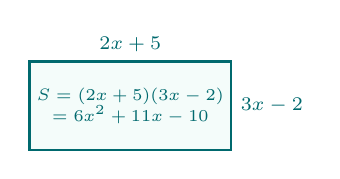
\begin{tikzpicture}[scale=0.80]
      \draw[thick, fill=brandTealBg, draw=koreaDarkTeal] (0,0) rectangle (3.2,1.4);
      \node[above, font=\fontsize{7.5}{7.5}\selectfont, color=brandNavy] at (1.6,1.4) {$2x + 5$};
      \node[right, font=\fontsize{7.5}{7.5}\selectfont, color=brandNavy] at (3.2,0.7) {$3x - 2$};
      \node[align=center, font=\fontsize{6.5}{7.5}\selectfont\kml, color=koreaDarkTeal] at (1.6,0.7) {
        $S = (2x+5)(3x-2)$\\
        $= 6x^2 + 11x - 10$
      };
    \end{tikzpicture}
  \end{minipage}
\end{khboxorange}

\begin{khcard}
  \textbf{\color{brandNavy}\ding{46}\ ឧទាហរណ៍គំរូ និងគំនូសបំព្រួញ ៖}\\[1.5pt]
  \noindent
  \begin{minipage}[t]{0.54\textwidth}
    \textbf{  	\color{blue}១. ការពន្លាតតាមគំនូសព្រួញ (FOIL Method) ៖}\\[1pt]
    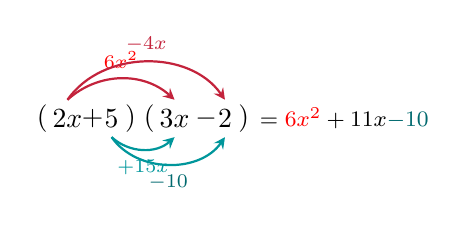
\begin{tikzpicture}[baseline=(base.center), scale=0.80]
      % Nodes for the expression
      \node (x1) at (0.35, 0) {$2x$};
      \node (p1) at (0.75, 0) {$+$};
      \node (y1) at (1.05, 0) {$5$};
      \node (b1) at (-0.05, 0) {$($};
      \node (b2) at (1.35, 0) {$)$};
      \node (b3) at (1.65, 0) {$($};
      \node (x2) at (2.05, 0) {$3x$};
      \node (m1) at (2.55, 0) {$-$};
      \node (y2) at (2.85, 0) {$2$};
      \node (b4) at (3.15, 0) {$)$};
      
      % Top arrows from 2x
      \draw[->, >=stealth, thick, color=brandCrimson] (x1.north) to[bend left=42] node[above, font=\fontsize{6.5}{6.5}\selectfont, color=brandCrimson] {\scriptsize ${\color{red}6x^2}$} (x2.north);
      \draw[->, >=stealth, thick, color=brandCrimson] (x1.north) to[bend left=55] node[above, font=\fontsize{6.5}{6.5}\selectfont, color=brandCrimson] {\scriptsize $-4x$} (y2.north);
      
      % Bottom arrows from 5
      \draw[->, >=stealth, thick, color=brandTeal] (y1.south) to[bend right=42] node[below, font=\fontsize{6.5}{6.5}\selectfont, color=brandTeal] {\scriptsize $+15x$} (x2.south);
      \draw[->, >=stealth, thick, color=brandTeal] (y1.south) to[bend right=55] node[below, font=\fontsize{6.5}{6.5}\selectfont, color=brandTeal] {\scriptsize ${\color{brandNavy}-10}$} (y2.south);
      
      \node[right, font=\fontsize{8.5}{8.5}\selectfont] at (3.25, 0) {$= {\color{red}6x^2} + 11x {\color{brandNavy}- 10}$};
      \node (base) at (0,0) {};
    \end{tikzpicture}
  \end{minipage}\hfill
  \begin{minipage}[t]{0.44\textwidth}
    \textbf{  	\color{blue}២. ការប្រើរូបមន្តសំខាន់ៗ ៖}\\[1.5pt]
    $\bullet\ \underbrace{({\color{red}2x}{\color{blue}+}3)^2}_{({\color{red}a}+b)^2} = \underbrace{({\color{red}2x})^2}_{{\color{red}a}^2} + \underbrace{2({\color{red}2x})(3)}_{2{\color{red}a}b} + \underbrace{3^2}_{b^2} = 4x^2 + 12x + 9$\\[2.5pt]
    $\bullet\ \underbrace{({\color{red}2x}+7)({\color{red}2x}-7)}_{({\color{red}a}+b)(a-b)} = ({\color{red}2x})^2 - 7^2 = 4x^2 - 49$
  \end{minipage}
\end{khcard}

\begin{multicols}{2}
  \columnseprule=0.5pt
  \def\columnseprulecolor{\color{koreaTeal!40}}

  \examplebadge{០១} ពន្លាត និងសម្រួលកន្សោម ៖
  \begin{enumerate}[label=\protect\khbadge{\kalph*}, leftmargin=18pt, itemsep=1.0pt, topsep=1pt]
    \item $A = 2x(3x - 5)$
    \item $B = (x + 3)(2x - 1)$
    \item $C = (x + 4)(x^2 - 4x + 1)$
    \item $D = (a - 2)(a^2 - 3a + 2) - a^2$ \hfill \examlabel
    \item $E = 4(x + 1)^2 - 9(2x - 1)^2$ \hfill \examlabel
    \item $F = -2(5x - 3)^2 + 3(4 + 3x)^2$ \hfill \examlabel
  \end{enumerate}

  \columnbreak

  \taskbadge{០១} ពន្លាត និងសម្រួល (ធ្វើខ្លួនឯង) ៖
  \begin{enumerate}[label=\protect\khbadge{\kalph*}, leftmargin=18pt, itemsep=1.0pt, topsep=1pt, start=7]
    \item $G = 3y(2y + 4)$
    \item $H = (3n + 4)(n + 5)$
    \item $I = (y + 5)(y^2 - 3y - 8)$
    \item $J = (x + 3)(x - 1)^2$
    \item $K = 3(4 + 3x)^2 - 2(5x - 3)^2$ \hfill \examlabel
    \item $L = (2x - 3)^3 + (2 + 3x)^3$ \hfill \examlabel
  \end{enumerate}

\end{multicols}

\vspace{1pt}
\begin{multicols}{2}
  \columnseprule=0.5pt
  \def\columnseprulecolor{\color{koreaTeal!40}}

  \examplebadge{០២} រក $a$ ដើម្បីឱ្យ ៖
  \begin{enumerate}[label=\protect\khbadge{\kalph*}, leftmargin=18pt, itemsep=0.8pt, topsep=0.5pt]
    \item $(x + a)(x - 8) = x^2 - 12x + 32$
    \item $(x + 3)(x + a) = x^2 + 7x + 12$
    \item $(x - 5)(x + a) = x^2 - 2x - 15$
    \item $(2x + a)(x - 3) = 2x^2 - x - 15$
  \end{enumerate}

  \columnbreak

  \taskbadge{០២} រក $a$ ដើម្បីឱ្យ (ធ្វើខ្លួនឯង) ៖
  \begin{enumerate}[label=\protect\khbadge{\kalph*}, leftmargin=18pt, itemsep=0.8pt, topsep=0.5pt, start=5]
    \item $(2y - 6)(y + a) = 2y^2 + 8y - 42$
    \item $(y + 4)(y + a) = y^2 + 9y + 20$
    \item $(y - 2)(y + a) = y^2 + 4y - 12$
    \item $(3y + a)(y + 2) = 3y^2 + 5y - 2$
  \end{enumerate}

\end{multicols}


% =========================================================================
% PAGE 3: SECTION 2 - FACTORING (COMMON FACTOR & GROUPING)
% =========================================================================
\khsection{២}{ការដាក់កន្សោមពិជគណិតជាផលគុណនៃកត្តា (Factoring Expressions)}

\khsubsection{២.១}{ដាក់ជាកត្តារួម និងវិធីផ្គុំតួ (Common Factor \& Grouping)}

\begin{khboxorange}
  \textbf{រូបមន្ត ៖} \koreahl{$ka \pm kb = k(a \pm b)$} \quad (ដែល $k$ ជាកត្តារួម អាចជាចំនួន អថេរ ឬកន្សោម)\\[2pt]
  \noindent
  \begin{minipage}[t]{0.48\textwidth}
    \textbf{១. ដាក់ជាកត្តារួម (ទាញតួដូចគ្នា) ៖}\\[1.5pt]
    $\bullet\ A = \mathbf{\textcolor{brandCrimson}{2x}} \cdot x + \mathbf{\textcolor{brandCrimson}{2x}} \cdot 2y = \mathbf{\textcolor{brandCrimson}{2x}}(x + 2y)$\\[2.5pt]
    $\bullet\ B = \mathbf{\textcolor{brandCrimson}{2(x - 1)}}[1 + 2(x - 1)] = 2(x - 1)(2x - 1)$
  \end{minipage}\hfill
  \begin{minipage}[t]{0.50\textwidth}
    \textbf{២. វិធីផ្គុំតួជាក្រុម (ស្វែងរកកត្តារួមថ្មី) ៖}\\[1.5pt]
    $C = \underbrace{(x^2 - x)}_{\textcolor{brandTeal}{x(x - 1)}} + \underbrace{(xy - y)}_{\textcolor{brandCrimson}{y(x - 1)}} = \mathbf{\textcolor{brandCrimson}{(x - 1)}}(x + y)$\\[2.5pt]
    \tikz[baseline]{\node[fill=white, draw=koreaTeal!50, rounded corners=2pt, inner sep=1.5pt, font=\fontsize{7.5}{7.5}\selectfont]{\textcolor{koreaDarkTeal}{\ding{228}\ បន្ទាប់ពីផ្គុំជា ២ ក្រុម ឃើញមានកត្តារួម $(x-1)$}};}
  \end{minipage}
\end{khboxorange}
\vspace{-0.2cm}
\begin{multicols}{2}
  \columnseprule=0.5pt
  \def\columnseprulecolor{\color{koreaTeal!40}}
  \examplebadge{០៣} ដាក់ជាផលគុណនៃកត្តា ៖\\[2pt]
  \noindent
  \begin{tabular}{@{}p{0.48\linewidth}@{\hspace{4pt}}p{0.48\linewidth}@{}}
    \khbadge{ក} $2x^4 + 8x$ & \khbadge{ខ} $7b^3 + 21b$ \\[4pt]
    \khbadge{គ} $8ax^2 - 12a^2x^3$ & \khbadge{ឃ} $10x^3y^2 - 15xy^3$ \\[4pt]
    \khbadge{ង} $4x^3 - 2x^2 + 14x$ & \khbadge{ច} $6x^2y - 9xy^2 + 12xy$
  \end{tabular}

  \columnbreak

  \taskbadge{០៣} ដាក់ជាផលគុណកត្តា (ធ្វើខ្លួនឯង) ៖\\[2pt]
  \noindent
  \begin{tabular}{@{}p{0.48\linewidth}@{\hspace{4pt}}p{0.48\linewidth}@{}}
    \khbadge{ឆ} $3y^4 + 9y$ & \khbadge{ជ} $5a^3 + 20a$ \\[4pt]
    \khbadge{ឈ} $6by^2 - 9b^2y^3$ & \khbadge{ញ} $12a^3b^2 - 18ab^3$ \\[4pt]
    \khbadge{ដ} $6y^3 - 3y^2 + 15y$ & \khbadge{ឋ} $8a^2b - 12ab^2 + 16ab$
  \end{tabular}

\end{multicols}

\vspace{1pt}
\begin{multicols}{2}
  \columnseprule=0.5pt
  \def\columnseprulecolor{\color{koreaTeal!40}}

  \examplebadge{០៤} ដាក់ជាផលគុណនៃកត្តា ៖
  \begin{enumerate}[label=\protect\khbadge{\kalph*}, leftmargin=18pt, itemsep=1.5pt, topsep=1pt]
    \item $a(x + 1) + b(x + 1) - c(x + 1)$ \hfill \examlabel
    \item $z(y - 3) + 2(y - 3)$
    \item $xy - 3x + 9y - 27$ \hfill \examlabel
    \item $ab + 7a + 4b + 28$
    \item $xy + 2x - 7y - 14$
    \item $ap - 2pk + ya - 2yk$
  \end{enumerate}

  \columnbreak

  \taskbadge{០៤} ដាក់ជាផលគុណកត្តា (ធ្វើខ្លួនឯង) ៖
  \begin{enumerate}[label=\protect\khbadge{\kalph*}, leftmargin=18pt, itemsep=1.5pt, topsep=1pt, start=7]
    \item $am - mb - an + nb$ \hfill \examlabel
    \item $12xy + 15x + 4y + 5$
    \item $2ab - 8a + 3b - 12$
    \item $3ab + 12a - b - 4$
    \item $xy - 8x - 3y + 24$
    \item $3x^2 - 6xy + 2ax - 4ay$
  \end{enumerate}

\end{multicols}

\vspace{1pt}
\begin{multicols}{2}
  \columnseprule=0.5pt
  \def\columnseprulecolor{\color{koreaTeal!40}}

  \examplebadge{០៥} ដាក់ជាផលគុណនៃកត្តា ៖
  \begin{enumerate}[label=\protect\khbadge{\kalph*}, leftmargin=18pt, itemsep=2pt, topsep=1pt]
    \item $A = at + bt + ct + 2a + 2b + 2c$
    \item $B = ax + 2ay + 3az - 4x - 8y - 12z$
  \end{enumerate}

  \columnbreak

  \taskbadge{០៥} ដាក់ជាផលគុណកត្តា (ធ្វើខ្លួនឯង) ៖
  \begin{enumerate}[label=\protect\khbadge{\kalph*}, leftmargin=18pt, itemsep=2pt, topsep=1pt, start=3]
    \item $C = ax + ay - az - bx - by + bz$
    \item $D = y^2 - cy - ay + ac - by + bc$
  \end{enumerate}

\end{multicols}



% =========================================================================
% PAGE 4: SECTION 2.2 - SPECIAL PRODUCT FORMULAS
% =========================================================================
\khsubsection{២.២}{ប្រើរូបមន្តសំខាន់ៗ (Special Product Formulas)}

\begin{khboxorange}
  \textbf{រូបមន្តសំខាន់ៗ ៖} \koreahl{$a^2 - b^2 = (a - b)(a + b)$} \quad \koreahl{$a^2 \pm 2ab + b^2 = (a \pm b)^2$} \quad \koreahl{$a^3 \pm b^3 = (a \pm b)(a^2 \mp ab + b^2)$}\\[2pt]
  \noindent
  \begin{minipage}[t]{0.48\textwidth}
    \textbf{១. ផលសងពីរការេ $a^2 - b^2 = (a-b)(a+b)$ ៖}\\[1pt]
    $\bullet\ 9x^2 - \dfrac{1}{4} = (3x)^2 - \left(\dfrac{1}{2}\right)^2 = \left(3x - \dfrac{1}{2}\right)\left(3x + \dfrac{1}{2}\right)$\\[2pt]
    $\bullet\ (2x-1)^2 - 9 = (2x-1-3)(2x-1+3) = 4(x-2)(x+1)$\\[2pt]
    $\bullet\ 4x^2(x+1) - 9(x+1) = (x+1)(2x-3)(2x+3)$
  \end{minipage}\hfill
  \begin{minipage}[t]{0.50\textwidth}
    \textbf{២. ការេនៃទ្វេធា និងផលបូក-ដកគូប ៖}\\[1pt]
    $\bullet\ 4x^2 - 12xy + 9y^2 = (2x)^2 - 2(2x)(3y) + (3y)^2 = (2x - 3y)^2$\\[2pt]
    $\bullet\ x^3 - 8 = x^3 - 2^3 = (x - 2)(x^2 + 2x + 4)$\\[2pt]
    $\bullet\ 27a^3 + 1 = (3a)^3 + 1^3 = (3a + 1)(9a^2 - 3a + 1)$
  \end{minipage}
\end{khboxorange}

\begin{multicols}{2}
  \columnseprule=0.5pt
  \def\columnseprulecolor{\color{koreaTeal!40}}

  \examplebadge{០៦} កំណត់តម្លៃនៃ $a$ \exambadge\ ៖
  \begin{enumerate}[label=\protect\khbadge{\kalph*}, leftmargin=18pt, itemsep=0.4pt, topsep=0.4pt]
    \item $4x^2 + 3ay^4 = (2x + 9y^2)(2x - 9y^2)$
  \end{enumerate}

  \columnbreak

  \taskbadge{០៦} កំណត់តម្លៃនៃ $a$ (ធ្វើខ្លួនឯង) \exambadge\ ៖
  \begin{enumerate}[label=\protect\khbadge{\kalph*}, leftmargin=18pt, itemsep=0.4pt, topsep=0.4pt, start=2]
    \item $16x^2 + 5ay^4 = (4x + 5y^2)(4x - 5y^2)$
  \end{enumerate}

\end{multicols}

\vspace{1pt}
\begin{multicols}{2}
  \columnseprule=0.5pt
  \def\columnseprulecolor{\color{koreaTeal!40}}

  \examplebadge{០៧} ដាក់ជាផលគុណនៃកត្តា ៖\\[2pt]
  \noindent
  \begin{tabular}{@{}p{0.48\linewidth}@{\hspace{4pt}}p{0.48\linewidth}@{}}
    \khbadge{ក} $x^2 - 16$ & \khbadge{ខ} $y^2 - 1$ \\[3.5pt]
    \khbadge{គ} $4x^2 - 49$ \hfill\examlabel & \khbadge{ឃ} $25x^2 - 9$ \hfill\examlabel \\[3.5pt]
    \khbadge{ង} $3x^2 - 75$ \hfill\examlabel & \khbadge{ច} $9x^2 - 4$ \hfill\examlabel \\[3.5pt]
    \khbadge{ឆ} $5x^2y^2 - 500$ & \khbadge{ជ} $2xy^2 - 32x$
  \end{tabular}

  \columnbreak

  \taskbadge{០៧} ដាក់ជាផលគុណកត្តា (ធ្វើខ្លួនឯង) ៖\\[2pt]
  \noindent
  \begin{tabular}{@{}p{0.48\linewidth}@{\hspace{4pt}}p{0.48\linewidth}@{}}
    \khbadge{ឈ} $y^2 - 121$ & \khbadge{ញ} $4m^2 - 144$ \\[3.5pt]
    \khbadge{ដ} $25b^2 - 64$ & \khbadge{ឋ} $t^4 - 1$ \\[3.5pt]
    \khbadge{ឌ} $4x^2 - 81$ \hfill\examlabel & \khbadge{ឍ} $16x^2 - 56x + 49$ \hfill\examlabel \\[3.5pt]
    \khbadge{ណ} $9x^2 + 12x + 4$ \hfill\examlabel & \khbadge{ត} $3a^2b^4 - 192a^3$
  \end{tabular}

\end{multicols}

\vspace{1pt}
\begin{multicols}{2}
  \columnseprule=0.5pt
  \def\columnseprulecolor{\color{koreaTeal!40}}

  \examplebadge{០៨} ដាក់ជាផលគុណនៃកត្តា ៖
  
  \begin{enumerate}[label=\protect\khbadge{\kalph*}, leftmargin=18pt, itemsep=0.8pt, topsep=0.5pt]
    \item $A = (x - y)^2 - 9z^2$ \hfill \examlabel
    \item $B = (x + y)^2 - (z + t)^2$
    \item $C = 9(x + 1)^2 - 25$ \hfill \examlabel
    \item $D = 9(x - 1)^2 - 4(2x + 3)^2$ \hfill \examlabel
    \item $E = (6x - 7)^2 - (2x - 7)^2$ \hfill \examlabel
    \item $F = (2x - 5)^2 - 4x^2 + 25$
    \item $G = 5ab^2 - 20a + 30b^2 - 120$
    \item $H = x^3 - x$
  \end{enumerate}

  \columnbreak

  \taskbadge{០៨} ដាក់ជាផលគុណកត្តា (ធ្វើខ្លួនឯង) ៖
  \begin{enumerate}[label=\protect\khbadge{\kalph*}, leftmargin=18pt, itemsep=0.8pt, topsep=0.5pt, start=9]
    \item $4(y + 2)^2 - y^2$
    \item $(a + b)^2 - (a - b)^2$
    \item $(2x + 1)^2 - (3x + 2)^2$ \hfill \examlabel
    \item $16(x + 3)^2 - (x - 1)^2$
    \item $(x + 1)^2 - (x^2 - 1) + 2x + 2$
    \item $4cx^2 - 4c - 12x^2 + 12$
    \item $2xy^2 - 2x + 4y^2 - 4$
    \item $x^5 - x$
    \item $8x^2 - 160x + 800$
  \end{enumerate}

\end{multicols}

\vspace{2pt}
\noindent
\begin{tcolorbox}[
  enhanced,
  colback=brandGoldBg,
  colframe=brandGold!50,
  arc=3pt,
  boxrule=0.6pt,
  left=6pt, right=6pt, top=3pt, bottom=3pt
]
  \noindent
  \begin{minipage}[t]{0.485\textwidth}
    \examplebadge{០៩} \textbf{កំណត់តម្លៃនៃ $m$ \exambadge\ ៖}\\[1pt]
    កំណត់តម្លៃនៃ $m$ ដើម្បីឱ្យ\\
    $A = 2x^3 + 3x^2 - 8x + 3 = (x - 1)(2x^2 + mx - 3)$\\
    រួចដាក់ $A$ ជាផលគុណកត្តាដឺក្រេទី ១។
  \end{minipage}\hfill\vline\hfill
  \begin{minipage}[t]{0.485\textwidth}
    \taskbadge{០៩} \textbf{កំណត់តម្លៃនៃ $m$ \exambadge\ ៖}\\[1pt]
    កំណត់តម្លៃនៃ $m$ ដើម្បីឱ្យ $x = 2$ ជាឫសនៃ\\
    សមីការ $x^2 - mx + 6 = 0$ រួចគណនាឫសមួយទៀត។
  \end{minipage}
\end{tcolorbox}

\clearpage

% =========================================================================
% PAGE 4: SECTION 2.3 & SECTION 3 - RATIONAL EXPRESSIONS
% =========================================================================
\khsubsection{២.៣}{វិធីគុណខ្វែង និងវិធីបំពេញបន្ថយតួ (Cross-Multiplication \& Completing Square)}

\begin{khboxorange}
  \textbf{១. វិធីគុណខ្វែង ៖} $ax^2 + bx + c = (a_1 x + c_1)(a_2 x + c_2)$ \quad \text{និង} \quad \textbf{២. វិធីបំពេញបន្ថយតួ ៖} $x^2 \pm 2ax = (x \pm a)^2 - a^2$\\[2pt]
  \noindent
  \begin{minipage}[t]{0.56\textwidth}
    \textbf{ឧទាហរណ៍គុណខ្វែង ៖}\\[1pt]
    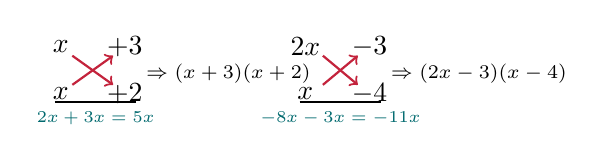
\begin{tikzpicture}[scale=0.74, baseline=(O.center)]
      \node (O) at (0,0.5) {};
      \node at (-0.2,0.9) {$x$}; \node at (0.9,0.9) {$+3$};
      \node at (-0.2,0.1) {$x$}; \node at (0.9,0.1) {$+2$};
      \draw[->, thick, color=brandCrimson] (0,0.75) -- (0.7,0.25);
      \draw[->, thick, color=brandCrimson] (0,0.25) -- (0.7,0.75);
      \draw[thick] (-0.3,-0.05) -- (1.1,-0.05);
      \node[below, font=\fontsize{6.5}{6.5}\selectfont, color=koreaDarkTeal] at (0.4,-0.05) {$2x+3x=5x$};
      \node[right, font=\fontsize{7.5}{7.5}\selectfont] at (1.1,0.45) {$\Rightarrow (x+3)(x+2)$};
      
      \begin{scope}[xshift=4.2cm]
        \node at (-0.2,0.9) {$2x$}; \node at (0.9,0.9) {$-3$};
        \node at (-0.2,0.1) {$x$}; \node at (0.9,0.1) {$-4$};
        \draw[->, thick, color=brandCrimson] (0.1,0.75) -- (0.7,0.25);
        \draw[->, thick, color=brandCrimson] (0.1,0.25) -- (0.7,0.75);
        \draw[thick] (-0.3,-0.05) -- (1.1,-0.05);
        \node[below, font=\fontsize{6.5}{6.5}\selectfont, color=koreaDarkTeal] at (0.4,-0.05) {$-8x-3x=-11x$};
        \node[right, font=\fontsize{7.5}{7.5}\selectfont] at (1.1,0.45) {$\Rightarrow (2x-3)(x-4)$};
      \end{scope}
    \end{tikzpicture}\\[3pt]
    $\bullet\ 3x^2 + 5x - 2 = (3x - 1)(x + 2)$ \hfill $\bullet\ x^2 - x - 12 = (x - 4)(x + 3)$
  \end{minipage}\hfill
  \begin{minipage}[t]{0.42\textwidth}
    \textbf{ឧទាហរណ៍បំពេញជាការេ ៖}\\[1pt]
    $\bullet\ x^2 - 2x - 8 = (x-1)^2 - 1^2 - 8 = (x-4)(x+2)$\\[2pt]
    $\bullet\ x^2 + 6x - 7 = (x+3)^2 - 3^2 - 7 = (x-1)(x+7)$\\[2pt]
    $\bullet\ x^4 + 4 = (x^2+2)^2 - (2x)^2 = (x^2-2x+2)(x^2+2x+2)$
  \end{minipage}
\end{khboxorange}

\begin{multicols}{2}
  \columnseprule=0.5pt
  \def\columnseprulecolor{\color{koreaTeal!40}}

  \examplebadge{១០} ដាក់ជាផលគុណនៃកត្តា ៖\\[2pt]
  \noindent
  \begin{tabular}{@{}p{0.48\linewidth}@{\hspace{4pt}}p{0.48\linewidth}@{}}
    \khbadge{ក} $x^2 + 5x + 6$ & \khbadge{ខ} $x^2 - 10x + 9$ \\[3.5pt]
    \khbadge{គ} $x^2 + 7x - 8$ & \khbadge{ឃ} $x^2 + 11x - 12$ \\[3.5pt]
    \khbadge{ង} $x^2 - xy - 30y^2$ \hfill\examlabel & \khbadge{ច} $a^2 - 3a - 18$ \\[3.5pt]
    \khbadge{ឆ} $n^2 - 4n - 12$ & \khbadge{ជ} $2x^2 + 5x - 3$ \\[3.5pt]
    \khbadge{ឈ} $m(m - 2) - 24$ \hfill\examlabel & \khbadge{ញ} $x^2 - 7x + 12$ \\[3.5pt]
    \khbadge{ដ} $x^2 - 2x - 15$ & \khbadge{ឋ} $3x^2 + 7x + 2$
  \end{tabular}

  \columnbreak

  \taskbadge{១០} ដាក់ជាផលគុណកត្តា (ធ្វើខ្លួនឯង) ៖\\[2pt]
  \noindent
  \begin{tabular}{@{}p{0.48\linewidth}@{\hspace{4pt}}p{0.48\linewidth}@{}}
    \khbadge{ឌ} $t^2 + 8t + 15$ & \khbadge{ឍ} $x^2 - 11x + 28$ \hfill\examlabel \\[3.5pt]
    \khbadge{ណ} $b^2 + 6b - 7$ & \khbadge{ត} $x^2 - 6x - 7$ \\[3.5pt]
    \khbadge{ថ} $y^2 - y - 12$ & \khbadge{ទ} $y^2 - 2y - 35$ \hfill\examlabel \\[3.5pt]
    \khbadge{ធ} $x^2 + 3x - 4$ & \khbadge{ន} $2x^2 + 13x - 7$ \\[3.5pt]
    \khbadge{ប} $m(m + 3) - 40$ \hfill\examlabel & \khbadge{ផ} $y^2 - 7y + 12$ \\[3.5pt]
    \khbadge{ព} $y^2 - 2y - 15$ & \khbadge{ភ} $3x^2 + 8x + 4$ \hfill\examlabel
  \end{tabular}

\end{multicols}

\vspace{-2pt}
\begin{multicols}{2}
  \columnseprule=0.5pt
  \def\columnseprulecolor{\color{koreaTeal!40}}

  \examplebadge{១១} ដាក់ជាផលគុណនៃកត្តា ៖\\[2pt]
  \noindent
  \begin{tabular}{@{}p{0.48\linewidth}@{\hspace{4pt}}p{0.48\linewidth}@{}}
    \khbadge{ក} $2a^2 + 24a + 70$ & \khbadge{ខ} $3x^2 + 21x + 36$ \\[3.5pt]
    \khbadge{គ} $5a^2 - 15a - 90$ & \khbadge{ឃ} $4x^2 - 8x - 60$ \\[3.5pt]
    \khbadge{ង} $2x^3 + 6x^2 - 20x$ & \khbadge{ច} $3y^3 - 3y^2 - 36y$ \\[3.5pt]
    \khbadge{ឆ} $ax^2 + 5ax + 6a$ & \khbadge{ជ} $2x^2y - 14xy + 20y$
  \end{tabular}

  \columnbreak

  \taskbadge{១១} ដាក់ជាផលគុណកត្តា (ធ្វើខ្លួនឯង) ៖\\[2pt]
  \noindent
  \begin{tabular}{@{}p{0.48\linewidth}@{\hspace{4pt}}p{0.48\linewidth}@{}}
    \khbadge{ឈ} $2x^2 - 4x - 160$ & \khbadge{ញ} $4bc^2 + 12bc - 40b$ \\[3.5pt]
    \khbadge{ដ} $6xy^4 + 18xy^2 - 168x$ & \khbadge{ឋ} $4y^2 - 8y - 96$ \\[3.5pt]
    \khbadge{ឌ} $3x^3 + 9x^2 - 30x$ & \khbadge{ឍ} $2t^3 - 2t^2 - 24t$ \\[3.5pt]
    \khbadge{ណ} $mx^2 + 5mx + 6m$ & \khbadge{ត} $3x^2y - 21xy + 30y$
  \end{tabular}

\end{multicols}

% -------------------------------------------------------------------------
% SECTION 3: RATIONAL EXPRESSIONS
% -------------------------------------------------------------------------
\vspace{-4pt}
\khsection{៣}{ប្រមាណវិធីលើកន្សោមសនិទាន (Rational Algebraic Expressions)}

\begin{khboxorange}
  \textbf{វិធានគណនា និងសម្រួលកន្សោមសនិទាន ៖}\\[1pt]
  \textbf{១.} ដាក់ភាគយកនិងភាគបែងជាផលគុណកត្តា \hfill \textbf{២.} សម្រួលកត្តាដូចគ្នា (លក្ខខណ្ឌខុសពី $0$)\\
  \textbf{៣.} រកភាគបែងរួម (LCM) រួចធ្វើប្រមាណវិធី \hfill \textbf{៤.} សម្រួលលទ្ធផលចុងក្រោយឱ្យសាមញ្ញបំផុត
\end{khboxorange}

\begin{khcard}
  \textbf{\color{brandNavy}\ding{46}\ ឧទាហរណ៍គំរូ និងជំហានគណនាលម្អិត ៖}\\[2pt]
  \noindent
  \begin{minipage}[t]{0.52\textwidth}
    \textbf{១. ផលបូក-ដកកន្សោមសនិទាន (តម្រូវភាគបែង) ៖}\\[1pt]
    គណនា $A = \dfrac{1}{(x+1)^2} + \dfrac{1}{x^2-1}$\\[2pt]
    \tikz[baseline]{\node[fill=brandCrimson!10, text=brandCrimson, rounded corners=2pt, inner sep=1.5pt, font=\fontsize{7}{7}\selectfont\bfseries]{១. រកភាគបែងរួម};} $x^2-1=(x-1)(x+1) \implies \text{LCD}=(x+1)^2(x-1)$\\[2pt]
    \tikz[baseline]{\node[fill=brandTeal!10, text=koreaDarkTeal, rounded corners=2pt, inner sep=1.5pt, font=\fontsize{7}{7}\selectfont\bfseries]{២. តម្រូវភាគបែង};} $A = \dfrac{\mathbf{\textcolor{brandCrimson}{(x-1)}}}{(x+1)^2\mathbf{\textcolor{brandCrimson}{(x-1)}}} + \dfrac{\mathbf{\textcolor{brandTeal}{(x+1)}}}{(x+1)^2(x-1)}$\\[2pt]
    \tikz[baseline]{\node[fill=brandNavy!10, text=brandNavy, rounded corners=2pt, inner sep=1.5pt, font=\fontsize{7}{7}\selectfont\bfseries]{៣. បូក និងសម្រួល};} $A = \dfrac{(x-1) + (x+1)}{(x+1)^2(x-1)} = \dfrac{\mathbf{2x}}{\mathbf{(x+1)^2(x-1)}}$
  \end{minipage}\hfill
  \begin{minipage}[t]{0.46\textwidth}
    \textbf{២. វិធីសម្រួលប្រភាគជាន់ (Complex Fraction) ៖}\\[1pt]
    សម្រួល $B = \dfrac{\dfrac{1}{x} - \dfrac{1}{y}}{\dfrac{1}{xy}}$ \quad (\text{ភាគបែងរួមនៃប្រភាគតូចគឺ} $xy$)\\[2pt]
    \tikz[baseline]{\node[fill=brandGold!20, text=brandGold!80!black, rounded corners=2pt, inner sep=1.5pt, font=\fontsize{7}{7}\selectfont\bfseries]{\ding{228}\ គុណភាគយក និងភាគបែងធំនឹង $xy$};}\\[2pt]
    $B = \dfrac{\left(\dfrac{1}{x} - \dfrac{1}{y}\right)\cdot \mathbf{\textcolor{brandCrimson}{xy}}}{\left(\dfrac{1}{xy}\right)\cdot \mathbf{\textcolor{brandCrimson}{xy}}} = \dfrac{\dfrac{1}{x}\cdot xy - \dfrac{1}{y}\cdot xy}{1} = \mathbf{y - x}$
  \end{minipage}

  \vspace{2pt}\hrule\vspace{2pt}
  \noindent
  \begin{minipage}[t]{0.54\textwidth}
    \textbf{៣. ផលគុណ និងផលចែកកន្សោមសនិទាន ៖}\\[1.5pt]
    $\bullet\ \dfrac{x^2 - 9}{x^2 + 2x} \cdot \dfrac{x+2}{x-3} = \dfrac{(x-3)(x+3)}{x(x+2)} \cdot \dfrac{x+2}{x-3} = \mathbf{\dfrac{x+3}{x}}$\\[2.5pt]
    $\bullet\ \dfrac{a^2 - 4}{a+1} \div \dfrac{a-2}{a^2 - 1} = \dfrac{(a-2)(a+2)}{a+1} \cdot \dfrac{(a-1)(a+1)}{a-2} = \mathbf{(a+2)(a-1)}$
  \end{minipage}\hfill
  \begin{minipage}[t]{0.44\textwidth}
    \textbf{៤. លក្ខខណ្ឌដើម្បីឱ្យកន្សោមសនិទានមានន័យ ៖}\\[1.5pt]
    កន្សោម $\dfrac{P(x)}{Q(x)}$ មានន័យលុះត្រាតែភាគបែង $Q(x) \neq 0$ ។\\[2pt]
    \textbf{ឧទាហរណ៍ ៖} រកលក្ខខណ្ឌនៃកន្សោម $E = \dfrac{2x - 5}{x^2 - 4x + 3}$\\[1.5pt]
    $x^2 - 4x + 3 \neq 0 \iff (x - 1)(x - 3) \neq 0 \iff \mathbf{x \neq 1 \ \text{និង}\ x \neq 3}$
  \end{minipage}
\end{khcard}

\clearpage

% =========================================================================
% PAGE 5: SECTION 3 EXERCISES
% =========================================================================
\begin{multicols}{2}
  \columnseprule=0.5pt
  \def\columnseprulecolor{\color{koreaTeal!40}}

  \examplebadge{១២} គណនាកន្សោមសនិទាន ៖\\[2pt]
  \noindent
  \begin{tabular}{@{}p{0.48\linewidth}@{\hspace{4pt}}p{0.48\linewidth}@{}}
    \khbadge{ក} $3x - \dfrac{x + 2}{x}$ & \khbadge{ខ} $y + \dfrac{y - 4}{3y + 4}$ \\[7pt]
    \khbadge{គ} $a - 3 - \dfrac{5}{a + 1}$ & \khbadge{ឃ} $\dfrac{t}{2(t + 3)} - \dfrac{2}{3(t + 3)}$ \\[7pt]
    \khbadge{ង} $\dfrac{6x - 1}{81 - x^2} - \dfrac{2x}{x + 9}$ & \khbadge{ច} $\dfrac{4z + 2}{16 - z^2} + \dfrac{4}{z - 4}$ \\[7.5pt]
    \multicolumn{2}{@{}l@{}}{\khbadge{ឆ} $\dfrac{ab^2 - b^2}{a(a+b)^2} \div \dfrac{b^2}{a(a^2-b^2)}$ \hfill\examlabel} \\[7.5pt]
    \multicolumn{2}{@{}l@{}}{\khbadge{ជ} $\dfrac{5x-2}{x^2-4} - \dfrac{3}{x+2} + \dfrac{x}{x-2}$ \hfill\examlabel}
  \end{tabular}

  \columnbreak

  \taskbadge{១២} គណនាកន្សោមសនិទាន (ធ្វើខ្លួនឯង) ៖\\[2pt]
  \noindent
  \begin{tabular}{@{}p{0.48\linewidth}@{\hspace{4pt}}p{0.48\linewidth}@{}}
    \khbadge{ឈ} $\dfrac{2x - 5}{3x} + 3x - 1$ & \khbadge{ញ} $3n + \dfrac{2n + 3}{4n + 5}$ \\[7pt]
    \khbadge{ដ} $b + 5 + \dfrac{5}{b - 5}$ & \khbadge{ឋ} $\dfrac{4x + 16}{x^2 - 16} - \dfrac{4}{x + 4}$ \\[7pt]
    \khbadge{ឌ} $\dfrac{10y - 1}{100 - y^2} - \dfrac{5y}{y + 10}$ & \khbadge{ឍ} $\dfrac{11}{121 - x^2} - \dfrac{x^2}{x + 11}$ \\[7.5pt]
    \multicolumn{2}{@{}l@{}}{\khbadge{ណ} $\dfrac{xy^2 - y^2}{x(x+y)^2} \div \dfrac{y^2}{x(x^2-y^2)}$ \hfill\examlabel} \\[7.5pt]
    \multicolumn{2}{@{}l@{}}{\khbadge{ត} $\dfrac{3a-6b}{a+b} - \dfrac{5a-6b}{a-b} - \dfrac{4a-5b}{a+b} + \dfrac{7a-8b}{a-b}$ \hfill\examlabel}
  \end{tabular}

\end{multicols}

\vspace{-2pt}
\begin{multicols}{2}
  \columnseprule=0.5pt
  \def\columnseprulecolor{\color{koreaTeal!40}}

  \examplebadge{១៣} វិញ្ញាសាប្រឡងឌីប្លូមគំរូ \exambadge\ ៖\\[1.5pt]
  គេឱ្យកន្សោមសនិទាន $A = \dfrac{x^2 - 9}{x^2 - 6x + 9}$ ។
  \begin{enumerate}[label=\protect\khbadge{\kalph*}, leftmargin=18pt, itemsep=0.3pt, topsep=0.2pt]
    \item រកលក្ខខណ្ឌនៃ $x$ ដើម្បីឱ្យកន្សោម $A$ មានន័យ
    \item សម្រួលកន្សោម $A$ 
    \item គណនាតម្លៃនៃ $A$ ចំពោះ $x = 5$
    \item រកតម្លៃនៃ $x$ ដើម្បីឱ្យកន្សោម $A = 2$
  \end{enumerate}
\vspace{-0.2cm}
  \columnbreak

  \taskbadge{១៣} កិច្ចការវិញ្ញាសាឌីប្លូម (ធ្វើខ្លួនឯង) \exambadge\ ៖\\[1.5pt]
  គេឱ្យកន្សោមសនិទាន $B = \dfrac{x^2 - 16}{x^2 - 8x + 16}$ ។
  \begin{enumerate}[label=\protect\khbadge{\kalph*}, leftmargin=18pt, itemsep=0.3pt, topsep=0.2pt, start=5]
    \item រកលក្ខខណ្ឌនៃ $x$ ដើម្បីឱ្យកន្សោម $B$ មានន័យ
    \item សម្រួលកន្សោម $B$ 
    \item គណនាតម្លៃនៃ $B$ ចំពោះ $x = 6$
    \item រកតម្លៃនៃ $x$ ដើម្បីឱ្យកន្សោម $B = 3$
  \end{enumerate}

\end{multicols}

\vspace{-2pt}
\begin{multicols}{2}
  \columnseprule=0.5pt
  \def\columnseprulecolor{\color{koreaTeal!40}}

  \examplebadge{១៤} សម្រួលកន្សោមសនិទាន ៖\\[2pt]
  \noindent
  \begin{tabular}{@{}p{0.48\linewidth}@{\hspace{4pt}}p{0.48\linewidth}@{}}
    \khbadge{ក} $\dfrac{\dfrac{1}{x} - \dfrac{3}{y}}{\dfrac{4}{y}}$ & \khbadge{ខ} $\dfrac{\dfrac{4}{x} + 5}{\dfrac{5}{y}}$ \\[10pt]
    \khbadge{គ} $\dfrac{\dfrac{1}{x} - \dfrac{1}{y}}{-\dfrac{6}{5y}}$ & \khbadge{ឃ} $\dfrac{1}{a + \dfrac{1}{a + \dfrac{1}{a}}}$ \\[12pt]
    \khbadge{ង} $\dfrac{1 - \dfrac{4}{x^2}}{1 + \dfrac{2}{x}}$ & \khbadge{ច} $\dfrac{\dfrac{a}{b} - \dfrac{b}{a}}{\dfrac{1}{a} + \dfrac{1}{b}}$ \\[10pt]
    \multicolumn{2}{@{}l@{}}{\khbadge{ឆ} $\dfrac{\dfrac{3x}{x^2 - 49} + \dfrac{7}{x + 7}}{\dfrac{1}{x - 7} - \dfrac{7}{2x + 14}}$}
  \end{tabular}

  \columnbreak

  \taskbadge{១៤} សម្រួលកន្សោមសនិទាន (ធ្វើខ្លួនឯង) ៖\\[2pt]
  \noindent
  \begin{tabular}{@{}p{0.48\linewidth}@{\hspace{4pt}}p{0.48\linewidth}@{}}
    \khbadge{ជ} $\dfrac{\dfrac{2}{x} + \dfrac{3}{y}}{\dfrac{5}{x}}$ & \khbadge{ឈ} $\dfrac{\dfrac{8}{x} - 9}{\dfrac{6}{y}}$ \\[10pt]
    \khbadge{ញ} $\dfrac{\dfrac{4}{a^2} + \dfrac{b}{a}}{\dfrac{2}{a} - 12}$ & \khbadge{ដ} $\dfrac{2}{c + \dfrac{1}{1 + \dfrac{c+1}{5-c}}}$ \\[12pt]
    \khbadge{ឋ} $\dfrac{1 - \dfrac{9}{y^2}}{1 + \dfrac{3}{y}}$ & \khbadge{ឌ} $\dfrac{\dfrac{x}{y} - \dfrac{y}{x}}{\dfrac{1}{y} - \dfrac{1}{x}}$ \\[10pt]
    \multicolumn{2}{@{}l@{}}{\khbadge{ឍ} $\dfrac{\dfrac{2b}{b - 4} - \dfrac{3}{b^2}}{\dfrac{5}{5b - 20} + \dfrac{3}{4b^2 - 16b}}$}
  \end{tabular}

\end{multicols}

\vspace{-2pt}
\begin{multicols}{2}
  \columnseprule=0.5pt
  \def\columnseprulecolor{\color{koreaTeal!40}}

  \examplebadge{១៥} កំណត់ចំនួនពិត $a, b, c$ ៖\\[1.5pt]
  ដើម្បីឱ្យ $\dfrac{2x^2 - x + 3}{x - 1} = ax + b + \dfrac{c}{x - 1}$

  \columnbreak

  \taskbadge{១៥} កំណត់ចំនួនពិត $m, n, p$ (ធ្វើខ្លួនឯង) ៖\\[1.5pt]
  ដើម្បីឱ្យ $\dfrac{3x^2 + 5x - 4}{x + 1} = mx + n + \dfrac{p}{x + 1}$

\end{multicols}

\clearpage

% =========================================================================
% PAGE 6: SECTION 4 - DIPLOMA EXAM PAPERS (POLYNOMIALS & FACTORING)
% =========================================================================
\koreanheader{វិញ្ញាសាឌីប្លូម}{កន្សោមពិជគណិត និងការដាក់ជាផលគុណកត្តា}

\khsection{៤}{វិញ្ញាសាប្រឡងឌីប្លូមជ្រើសរើស (National Diploma Exam Papers)}

\begin{multicols}{2}
  \columnseprule=0.5pt
  \def\columnseprulecolor{\color{koreaTeal!40}}

  \examplebadge{១៦} \textbf{វិញ្ញាសាឌីប្លូម (២០ ពិន្ទុ)} \exambadge\ ៖\\[1.5pt]
  គេមានកន្សោម $A = 4(x - 1)^2 - 9(x + 2)^2$ ។
  \begin{enumerate}[label=\protect\khbadge{\kalph*}, leftmargin=18pt, itemsep=0.4pt, topsep=0.2pt]
    \item ពន្លាតកន្សោម $A$ រួចគណនា
    \item ដាក់កន្សោម $A$ ជាផលគុណកត្តាដឺក្រេទី ១ នៃ $x$
    \item ដោះស្រាយសមីការ $A = 0$
    \item គណនាតម្លៃនៃ $A$ ចំពោះ $x = 1$, $x = -2$
  \end{enumerate}

  \columnbreak

  \taskbadge{១៦} \textbf{កិច្ចការឌីប្លូម (២០ ពិន្ទុ)} \exambadge\ ៖\\[1.5pt]
  គេមានកន្សោម $P = 9x^2 - 16 - 2(3x + 4)(x - 3)$ ។
  \begin{enumerate}[label=\protect\khbadge{\kalph*}, leftmargin=18pt, itemsep=0.4pt, topsep=0.2pt, start=5]
    \item ពន្លាតកន្សោម $P$ រួចរៀបតាមដឺក្រេចុះនៃ $x$
    \item ដាក់កន្សោម $P$ ជាផលគុណកត្តាដឺក្រេទី ១ នៃ $x$
    \item ដោះស្រាយសមីការ $P = 0$
    \item គណនាតម្លៃនៃ $P$ ចំពោះ $x = -1$, $x = 2$
  \end{enumerate}

\end{multicols}

\vspace{-0.2cm}
\begin{multicols}{2}
  \columnseprule=0.5pt
  \def\columnseprulecolor{\color{koreaTeal!40}}

  \examplebadge{១៧} \textbf{វិញ្ញាសាឌីប្លូម (២០ ពិន្ទុ)} \exambadge\ ៖\\[1.5pt]
  គេឱ្យកន្សោម $A = (4x^2 - 25)^2 - (2x + 5)^2$ ។
  \begin{enumerate}[label=\protect\khbadge{\kalph*}, leftmargin=18pt, itemsep=0.4pt, topsep=0.2pt]
    \item ពន្លាត និងរៀប $A$ តាមលំដាប់ស្វ័យគុណចុះនៃ $x$
    \item សរសេរ $A$ ជាទម្រង់ផលគុណកត្តាដឺក្រេទី ១
    \item គណនាតម្លៃនៃ $A$ ចំពោះ $x = -1$, $x = 1$, $x = \sqrt{5}$
  \end{enumerate}

  \columnbreak
\vspace{-0.2cm}
  \taskbadge{១៧} \textbf{កិច្ចការឌីប្លូម (២០ ពិន្ទុ)} \exambadge\ ៖\\[1.5pt]
  គេឱ្យកន្សោម $P = (x - 2)(7 - 3x) - (x - 2)^2$ ។
  \begin{enumerate}[label=\protect\khbadge{\kalph*}, leftmargin=18pt, itemsep=0.4pt, topsep=0.2pt, start=4]
    \item ពន្លាត និងរៀប $P$ តាមលំដាប់ស្វ័យគុណចុះនៃ $x$
    \item ដាក់កន្សោម $P$ ជាផលគុណកត្តាដឺក្រេទី ១
    \item ដោះស្រាយសមីការ $P = 0$
    \item គណនាតម្លៃនៃ $P$ ចំពោះ $x = -1$, $x = 0$, $x = \dfrac{3}{4}$
  \end{enumerate}

\end{multicols}

\vspace{-2pt}
\begin{multicols}{2}
  \columnseprule=0.5pt
  \def\columnseprulecolor{\color{koreaTeal!40}}

  \examplebadge{១៨} \textbf{វិញ្ញាសាឌីប្លូម (២០ ពិន្ទុ)} \exambadge\ ៖\\[1.5pt]
  គេឱ្យកន្សោម $A = 16x^2 - 56x + 49$, $B = 25x^2 - 9$ និង $C = (6x - 7)^2 - (2x - 7)^2$ ។
  \begin{enumerate}[label=\protect\khbadge{\kalph*}, leftmargin=18pt, itemsep=0.4pt, topsep=0.2pt]
    \item ដាក់ $A, B, C$ ជាផលគុណកត្តាដឺក្រេទី ១
    \item សម្រួលប្រភាគ $D = \dfrac{C}{A}$
    \item គណនាតម្លៃ $D$ ចំពោះ $x = 0$, $x = 2$, $x = -5$
  \end{enumerate}

  \columnbreak

  \taskbadge{១៨} \textbf{កិច្ចការឌីប្លូម (២០ ពិន្ទុ)} \exambadge\ ៖\\[1.5pt]
  គេឱ្យកន្សោម $A = \dfrac{6x^2 - 4x}{9x^2 - 4}$, $B = \dfrac{9x + 6}{9x^2 + 12x + 4}$ និង $C = \dfrac{5x}{15x^2 + 10x}$ ។
  \begin{enumerate}[label=\protect\khbadge{\kalph*}, leftmargin=18pt, itemsep=0.4pt, topsep=0.2pt, start=4]
    \item បំបែកភាគបែង $9x^2 - 4$ និង $9x^2 + 12x + 4$ ជាកត្តា
    \item សម្រួលកន្សោម $A$, $B$ និង $C$
    \item គណនាផលបូក $S = A - B + C$
  \end{enumerate}

\end{multicols}

\vspace{1pt}
\noindent
\begin{tcolorbox}[
  enhanced,
  colback=brandTealBg,
  colframe=koreaTeal!60,
  arc=3.5pt,
  boxrule=0.7pt,
  left=8pt, right=8pt, top=4pt, bottom=4pt
]
  \fontsize{8.5}{9.5}\selectfont\kml
  \textcolor{koreaDarkTeal}{\ding{72}\ \textbf{វិធីសាស្ត្រដោះស្រាយកន្សោមពិជគណិតក្នុងវិញ្ញាសាប្រឡងឌីប្លូម ៖}}\\
  \textcolor{brandCrimson}{\ding{228}}\ \textbf{ការពន្លាត និងបង្រួម ៖} ប្រើប្រាស់រូបមន្ត $(a \pm b)^2 = a^2 \pm 2ab + b^2$ រួចបូកដកតួដូចគ្នា និងរៀបតាមដឺក្រេចុះ។\\
  \textcolor{brandCrimson}{\ding{228}}\ \textbf{ការដាក់ជាផលគុណកត្តា ៖} ពិនិត្យមើលកត្តារួម $(a-b)$ ឬទម្រង់ផលសងពីរការេ $A^2 - B^2 = (A-B)(A+B)$ ជានិច្ច។\\
  \textcolor{brandCrimson}{\ding{228}}\ \textbf{ការដោះស្រាយសមីការ $P = 0$ ៖} ត្រូវបំប្លែងកន្សោមទៅជាផលគុណកត្តា $A \cdot B = 0 \iff A = 0$ ឬ $B = 0$។
\end{tcolorbox}

\clearpage

% =========================================================================
% PAGE 8: SECTION 4 - DIPLOMA EXAM PAPERS (RATIONAL EXPRESSIONS) & BACK COVER
% =========================================================================
\koreanheader{វិញ្ញាសាឌីប្លូម}{ប្រមាណវិធី និងសម្រួលកន្សោមសនិទាន}

\begin{multicols}{2}
  \columnseprule=0.5pt
  \def\columnseprulecolor{\color{koreaTeal!40}}

  \examplebadge{១៩} \textbf{វិញ្ញាសាប្រឡងឌីប្លូម} \exambadge\ ៖\\[1.5pt]
  គេមានកន្សោម $A = 4x^2 - 64$ និង $B = x^2 + x - 12$ ។
  \begin{enumerate}[label=\protect\khbadge{\kalph*}, leftmargin=18pt, itemsep=0.4pt, topsep=0.2pt]
    \item ដាក់កន្សោម $A$ និង $B$ ជាផលគុណកត្តាដឺក្រេទី ១
    \item រកតម្លៃនៃ $x$ ដែលនាំឱ្យ $A = B$
    \item សម្រួលកន្សោម $F = \dfrac{A}{B}$
  \end{enumerate}

  \columnbreak

  \taskbadge{១៩} \textbf{កិច្ចការវិញ្ញាសាឌីប្លូម} \exambadge\ ៖\\[1.5pt]
  គេមានកន្សោមពីរ $A = 3x^2 - 75$ និង $B = x^2 - 2x - 35$ ។
  \begin{enumerate}[label=\protect\khbadge{\kalph*}, leftmargin=18pt, itemsep=0.4pt, topsep=0.2pt, start=4]
    \item ដាក់កន្សោម $A$ និង $B$ ជាផលគុណកត្តាដឺក្រេទី ១
    \item រកតម្លៃនៃ $x$ ដើម្បីឱ្យ $A = B$
    \item សម្រួលកន្សោម $F = \dfrac{A}{B}$
  \end{enumerate}

\end{multicols}

\vspace{-2pt}
\begin{multicols}{2}
  \columnseprule=0.5pt
  \def\columnseprulecolor{\color{koreaTeal!40}}

  \examplebadge{២០} \textbf{វិញ្ញាសាប្រឡងឌីប្លូម} \exambadge\ ៖\\[1.5pt]
  គេឱ្យកន្សោម $A = x^2(x + 1) - 25(x + 1)$ និង $B = x^2 + 6x + 5$ ។
  \begin{enumerate}[label=\protect\khbadge{\kalph*}, leftmargin=18pt, itemsep=0.4pt, topsep=0.2pt]
    \item ដាក់កន្សោម $A$ និង $B$ ជាផលគុណកត្តា
    \item សម្រួលកន្សោម $C = \dfrac{A}{B}$ រួចគណនាតម្លៃនៃ $C$ ចំពោះ $x = 2$
  \end{enumerate}

  \columnbreak

  \taskbadge{២០} \textbf{កិច្ចការវិញ្ញាសាឌីប្លូម} \exambadge\ ៖\\[1.5pt]
  គេមានពីរកន្សោម $A = 2x^3 - 12x^2 + 18x$ និង $B = 2x^2 - 18$ ។
  \begin{enumerate}[label=\protect\khbadge{\kalph*}, leftmargin=18pt, itemsep=0.4pt, topsep=0.2pt, start=3]
    \item ដាក់កន្សោម $A$ និង $B$ ជាផលគុណកត្តាដឺក្រេទី ១ នៃ $x$
    \item សម្រួលកន្សោម $F = \dfrac{A}{B}$ រួចរកលក្ខខណ្ឌដែលនាំឱ្យ $F$ មានន័យ
  \end{enumerate}

\end{multicols}

\vspace{-2pt}
\begin{multicols}{2}
  \columnseprule=0.5pt
  \def\columnseprulecolor{\color{koreaTeal!40}}

  \examplebadge{២១} \textbf{វិញ្ញាសាប្រឡងឌីប្លូម} \exambadge\ ៖\\[1.5pt]
  គេមានកន្សោម $M = x^2 - 4$ និង $N = 2x^2 - x - 6$ ។
  \begin{enumerate}[label=\protect\khbadge{\kalph*}, leftmargin=18pt, itemsep=0.4pt, topsep=0.2pt]
    \item ដាក់ $M$ និង $N$ ជាផលគុណនៃកត្តា
    \item សម្រួល $F = \dfrac{M}{N}$ រួចគណនា $F$ កាលណា $x = \sqrt{2}$
  \end{enumerate}

  \columnbreak

  \taskbadge{២១} \textbf{កិច្ចការវិញ្ញាសាឌីប្លូម} \exambadge\ ៖\\[1.5pt]
  គេឱ្យកន្សោម $M = 3x^2 + 7x - 6$ ។
  \begin{enumerate}[label=\protect\khbadge{\kalph*}, leftmargin=18pt, itemsep=0.4pt, topsep=0.2pt, start=3]
    \item សម្រួលប្រភាគ $F = \dfrac{M}{(x - 2)(x + 3)}$
    \item គណនាតម្លៃនៃ $F$ ចំពោះ $x = 3$
  \end{enumerate}

\end{multicols}

\vspace{-2pt}
\begin{multicols}{2}
  \columnseprule=0.5pt
  \def\columnseprulecolor{\color{koreaTeal!40}}

  \examplebadge{២២} \textbf{វិញ្ញាសាប្រឡងឌីប្លូម} \exambadge\ ៖\\[1.5pt]
  គេឱ្យកន្សោម ៖\\
  $A = (x+5)(x^2+3x-10)$\\
  $B = x^2(x-1) + 10x(x-1) + 25x - 25$ ។
  \begin{enumerate}[label=\protect\khbadge{\kalph*}, leftmargin=18pt, itemsep=0.4pt, topsep=0.2pt]
    \item ដាក់កន្សោម $A$ និង $B$ ជាផលគុណកត្តាដឺក្រេទី ១ នៃ $x$
    \item សម្រួលកន្សោម $F = \dfrac{A}{B}$
    \item គណនាតម្លៃលេខនៃ $F$ ចំពោះ $x = \sqrt{2}$
  \end{enumerate}

  \columnbreak

  \taskbadge{២២} \textbf{កិច្ចការស្វ័យសិក្សា} \exambadge\ ៖\\[1.5pt]
  គេឱ្យកន្សោម ៖\\
  $P = \dfrac{2x^3 - 8x}{2x^3 - 8x^2 + 8x}$ \quad \text{និង} \quad $Q = \dfrac{3x^3 - 27x}{3x^3 + 18x^2 + 27x}$ ។
  \begin{enumerate}[label=\protect\khbadge{\kalph*}, leftmargin=18pt, itemsep=0.4pt, topsep=0.2pt, start=4]
    \item សម្រួលកន្សោម $P$ និង $Q$
    \item គណនាតម្លៃនៃ $P$ និង $Q$ ចំពោះ $x = 2026$
  \end{enumerate}

\end{multicols}

\vspace{1pt}
\noindent
\begin{tcolorbox}[
  enhanced,
  colback=brandGoldBg,
  colframe=brandGold!50,
  arc=3.5pt,
  boxrule=0.7pt,
  left=8pt, right=8pt, top=4pt, bottom=4pt
]
  \fontsize{8.5}{9.5}\selectfont
  \textcolor{brandCrimson}{\ding{72}\ \textbf{ចំណាំសំខាន់ចំពោះការគណនាតម្លៃលេខកន្សោមសនិទាន ៖}}\\
  $\bullet$\ ពេលគេឱ្យគណនាតម្លៃកន្សោម $F$ ចំពោះ $x = \sqrt{2}$ ឬ $x = \text{ចំនួនអសនិទាន}$ ត្រូវសម្រួលកន្សោមឱ្យអស់ជាមុនសិន រួចទើបជំនួសតម្លៃ $x$ ចូល និងបំបាត់រ៉ាឌីកាល់ពីភាគបែង។
\end{tcolorbox}

\end{document}
